\chapter{Desarrollo}

\section{GeoKettle}
Como se puede ver en la figura \ref{fig:spoon-missing-plugins}, al importar las transformaciones creadas en
GeoKettle a PDI9, partes del workflow fallan. Es lo que se pretende solucionar.

\begin{figure}[H]
    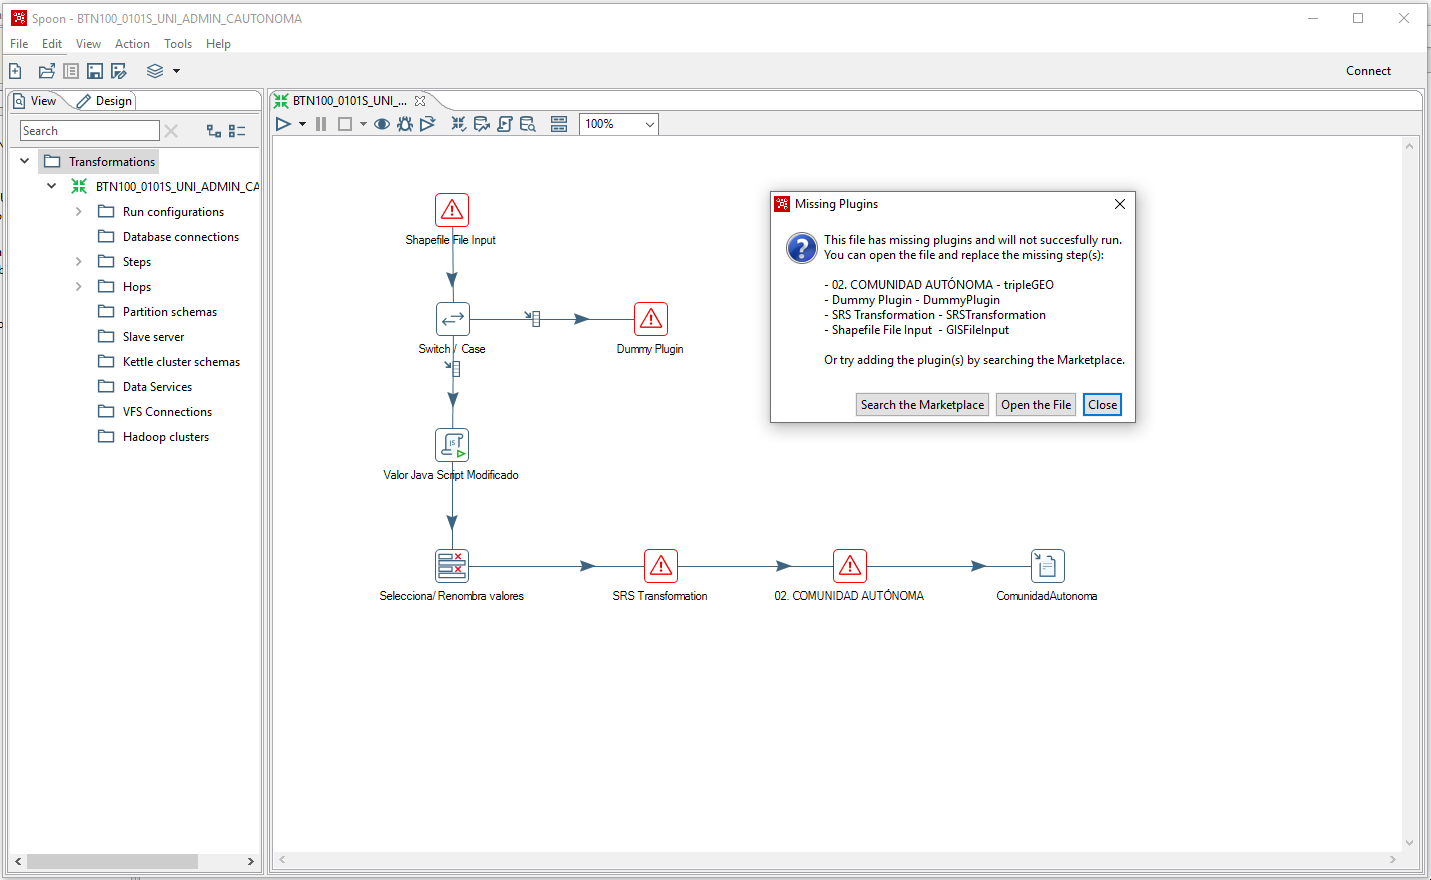
\includegraphics[width=\textwidth]{images/spoon-missing-plugins.png}
    \centering
    \caption{Workflow importado en la nueva suite}
    \label{fig:spoon-missing-plugins}
\end{figure}

\newpage
\subsection{Funcionamiento}

Para poder realizar el ``port'' de GeoKettle a Spoon, primero es necesario entender el funcionamiento y
transformaciones actuales de GeoKettle observando la entrada y salida de cada paso. Además esta manera se
observará mejor el flujo de datos y será más facil añadir soporte a GeoPackage en el futuro. No todas las
transformaciones tienen los mismos pasos, pero son parecidas. Como ejemplo se utilizarán los datos de
BTN100\_0101S\_UNI\_ADMIN y la transformación BTN100\_0101S\_UNI\_ADMIN\_CAUTONOMA. La transformación contiene
los siguientes pasos:

\begin{figure}[H]
    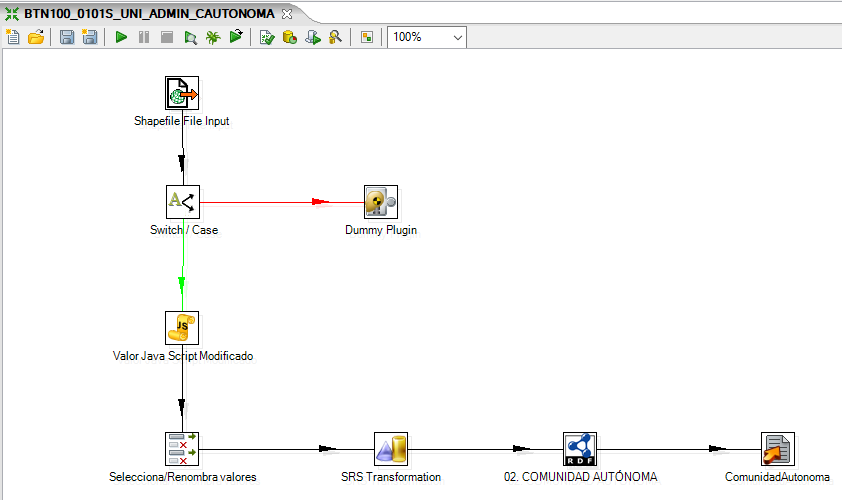
\includegraphics[width=\textwidth]{images/CCAA.png}
    \centering
    \caption{Transformación BTN100\_0101S\_UNI\_ADMIN\_CAUTONOMA}
    \label{fig:CCAA}
\end{figure}


\begin{enumerate}
    \item Shapefile File Input
    \item Switch Case
    \item Dummy Plugin
    \item Valor Java Script Modificado
    \item Selecciona/Renombra valores
    \item SRS Transformation
    \item TripleGeo
    \item Text Output
\end{enumerate}


\subsubsection{Shapefile File Input}

Lee el fichero shapefile.
\begin{enumerate}
    \item \textit{.shp}: Geometría fig.\ref{fig:shapefile}

        \begin{figure}[H]
            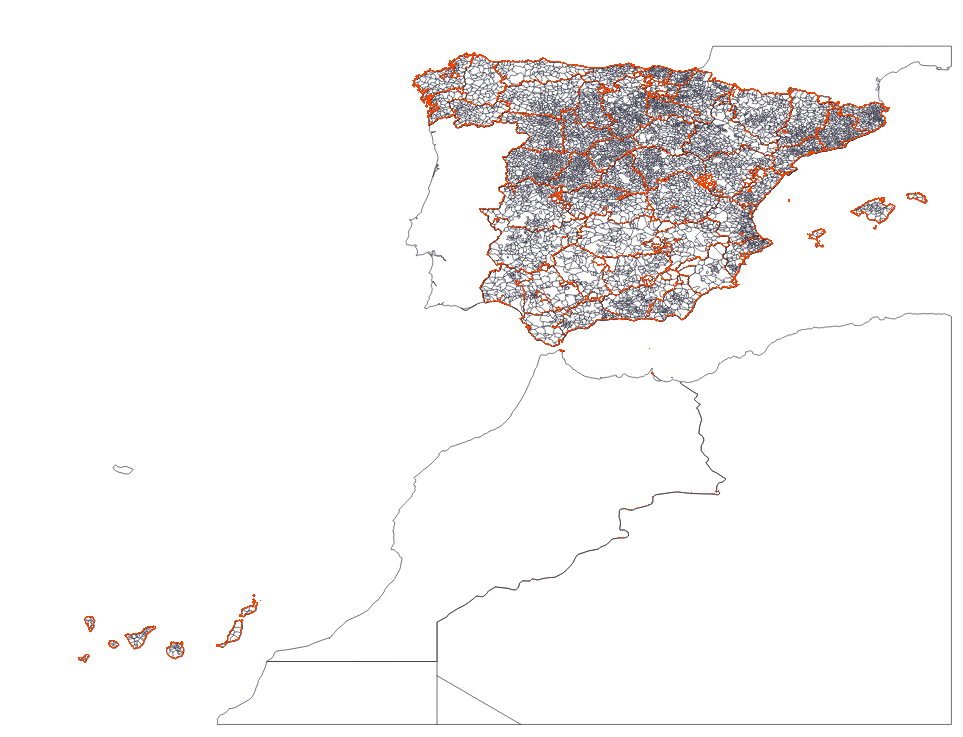
\includegraphics[width=0.7\textwidth]{images/shapefile.png}
            \centering
            \caption{Geometría contenida en el shapefile}
            \label{fig:shapefile}
        \end{figure}

    \item \textit{.dbf}: Datos asociados en columnas fig.\ref{fig:dbf}

        \begin{figure}[H]
            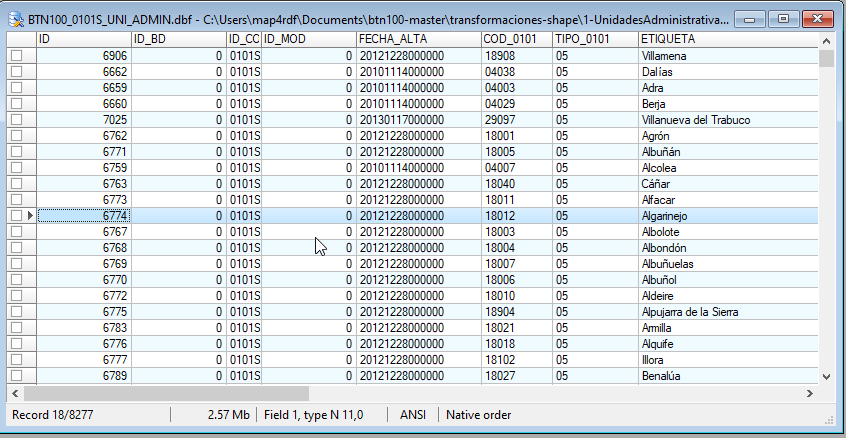
\includegraphics[width=0.7\textwidth]{images/dbf.png}
            \centering
            \caption{Datos columnares dbf asociados a la geometría}
            \label{fig:dbf}
        \end{figure}

    \item \textit{.shx}: Índice para acelerar búsquedas
    \item \textit{.prj}: Sistema de coordenadas
\end{enumerate}

\subsubsection{Switch case}
El switch case se encarga de filtrar y seleccionar las comunidades autónomas, identificadas por el valor 02 del
Campo TIPO\_0101. Si son una CCAA, se envían al paso 4, e.o.c. se envían al paso 3. fig.\ref{fig:switch} y
\ref{fig:tipo02}

\begin{figure}[H]
    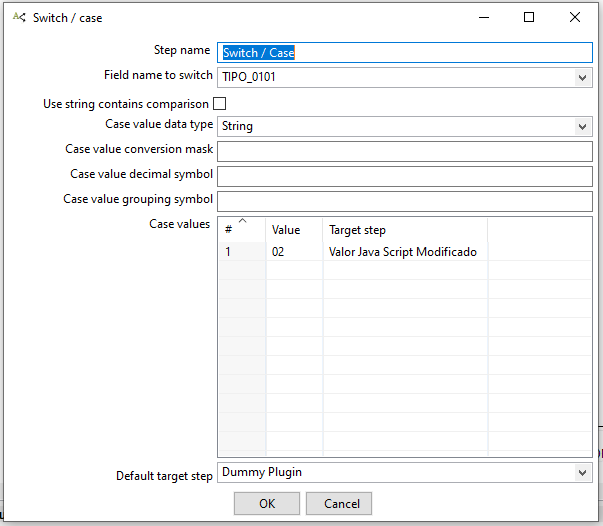
\includegraphics[width=0.7\textwidth]{images/switch.png}
    \centering
    \caption{Paso switch}
    \label{fig:switch}
\end{figure}

\begin{figure}[H]
    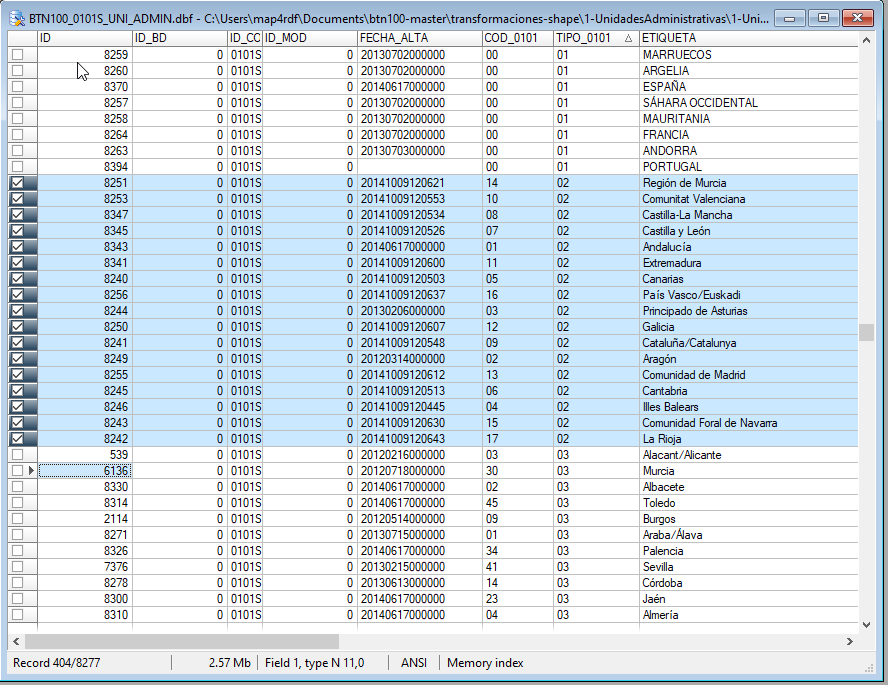
\includegraphics[width=\textwidth]{images/tipo02.png}
    \centering
    \caption{La filas correspondientes a las CCAA}
    \label{fig:tipo02}
\end{figure}

\subsubsection{Dummy Plugin}
No hace ninguna transformación, su propósito es recoger los datos innecesarios del switch.

\subsubsection{Valor Java Script Modificado}
El script cambia el formato de la fecha para facilitar la lectura: de YYYYMMDDHHMMSS a YYYY-MM-DD. También
crea un nuevo campo llamado identificador a partir del campo etiqueta, cambiando espacios por barras bajas, mayúsculas
por minúsculas, quitando tildes y signos de puntuación. fig.\ref{fig:script} y \ref{fig:fecha}

\begin{figure}[H]
    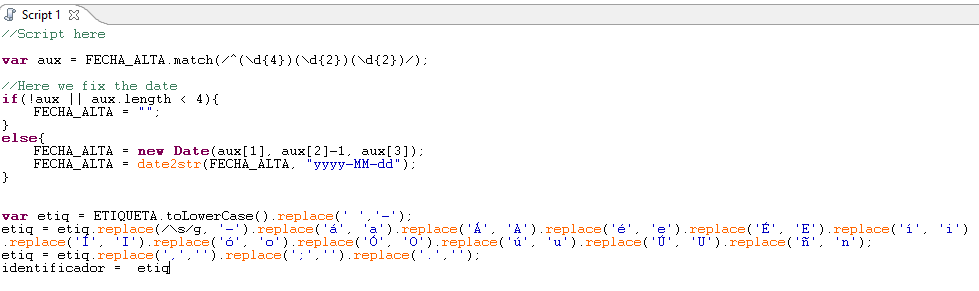
\includegraphics[width=\textwidth]{images/script.png}
    \centering
    \caption{Script Javascript}
    \label{fig:script}
\end{figure}

\begin{figure}[H]
    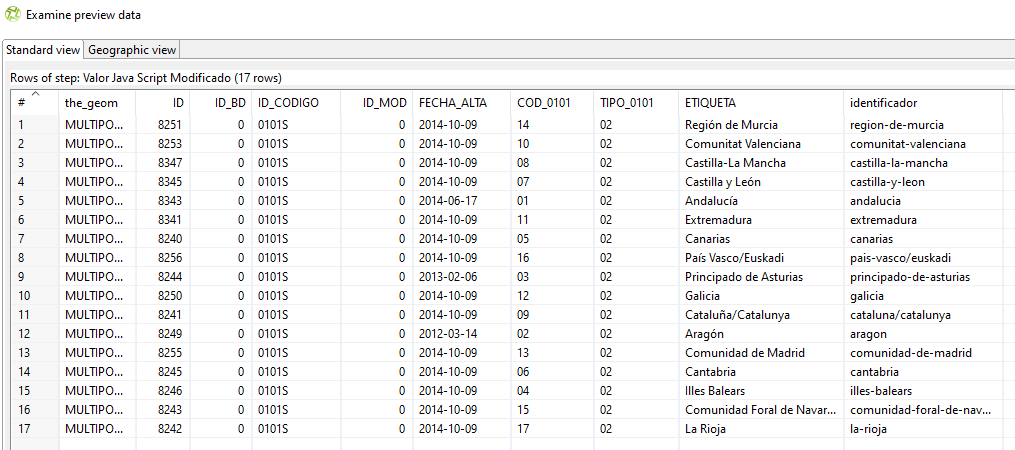
\includegraphics[width=\textwidth]{images/fecha.png}
    \centering
    \caption{Resultado del cambio de formato de fecha}
    \label{fig:fecha}
\end{figure}

\subsubsection{Selecciona/Renombra valores}
Cambia los metadatos de la columna FECHA\_ALTA para que sea reconocida como fecha. fig.\ref{fig:selecciona-renombra}

\begin{figure}[H]
    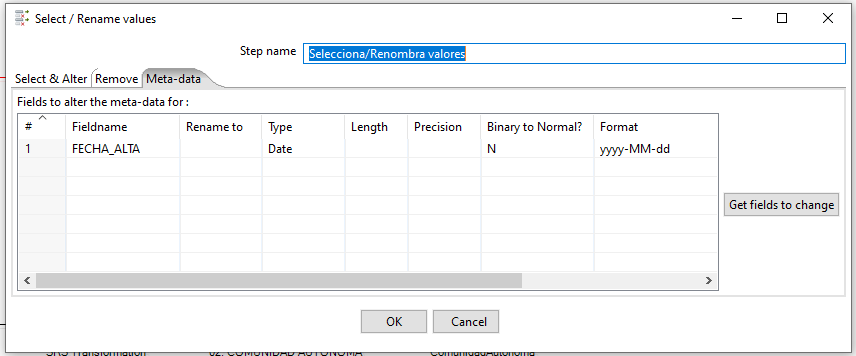
\includegraphics[width=\textwidth]{images/selecciona-renombra.png}
    \centering
    \caption{Selecciona/renombra valores}
    \label{fig:selecciona-renombra}
\end{figure}

\subsubsection{SRS Transformation}
Realiza la reproyección del sistema de coordenadas, en este caso de ETRS89 a WGS84. fig.\ref{fig:SRS}

\begin{figure}[H]
    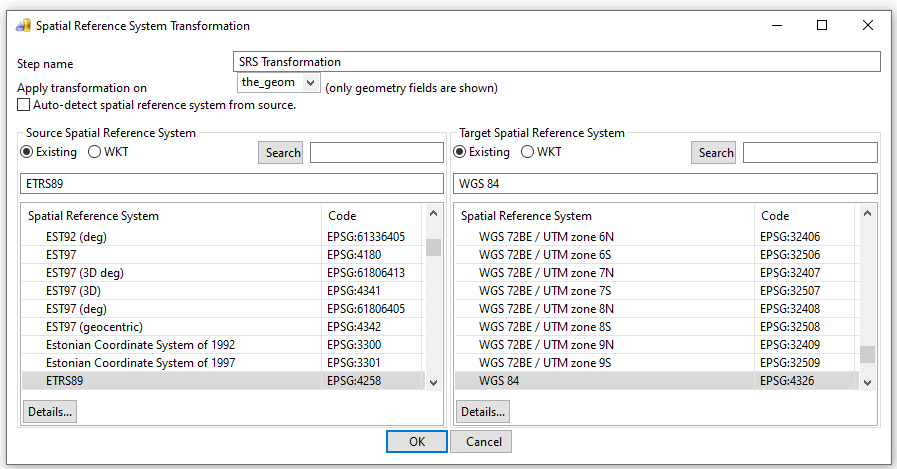
\includegraphics[width=\textwidth]{images/SRS.png}
    \centering
    \caption{Transformacion SRS}
    \label{fig:SRS}
\end{figure}

\subsubsection{TripleGeoKettle}
Transforma el shapefile del paso anterior en RDF en formato ttl. Se pueden configurar los parámetros asociados a la
ontologia y decidir si se muestran ciertas columnas o no. fig.\ref{fig:tripleGeoKettle}


\begin{figure}[H]
    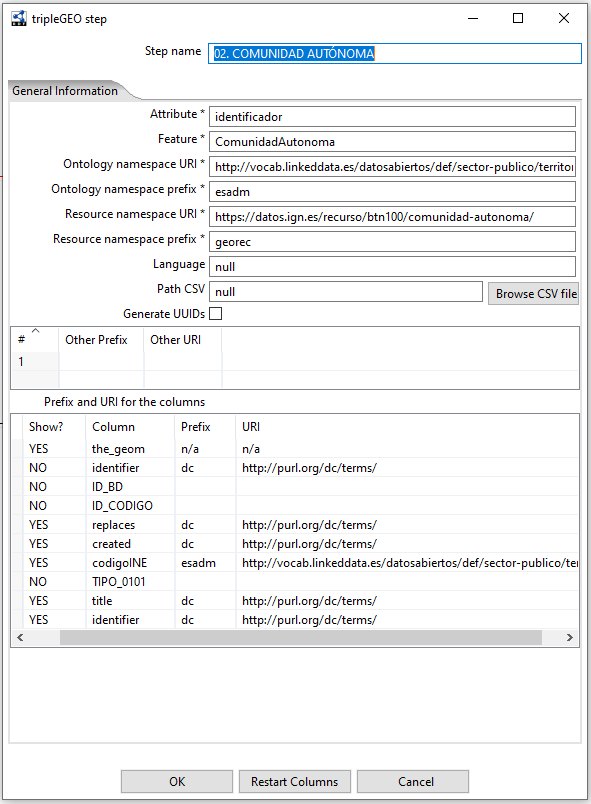
\includegraphics[width=0.9\textwidth]{images/tripleGeoKettle.png}
    \centering
    \caption{tripleGeoKettle}
    \label{fig:tripleGeoKettle}
\end{figure}

\subsubsection{Text file output}
Escribe los datos RDF en un fichero de texto con formato .ttl. fig.\ref{fig:text-file-output}
\begin{figure}[H]
    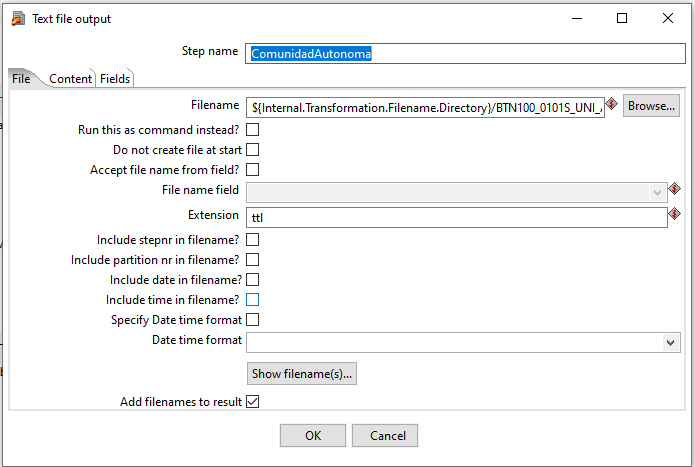
\includegraphics[width=\textwidth]{images/text-file-output.png}
    \centering
    \caption{text-file-output}
    \label{fig:text-file-output}
\end{figure}

\subsubsection{Resultado de la transformación}

El resultado es un ttl que sigue la ontologia definida, y tiene integrados los datos del shapefile que se han
seleccionado, incluso las geometrías.

\footnotesize
\begin{verbatim}
@prefix geo:   <http://www.w3.org/2003/01/geo/wgs84_pos#> .
@prefix geosparql: <http://www.opengis.net/ont/geosparql#> .
@prefix sf:    <http://www.opengis.net/ont/sf#> .
@prefix rdf:   <http://www.w3.org/1999/02/22-rdf-syntax-ns#> .
@prefix owl:   <http://www.w3.org/2002/07/owl#> .
@prefix xsd:   <http://www.w3.org/2001/XMLSchema#> .
@prefix georec: <https://datos.ign.es/recurso/btn100/comunidad-autonoma/> .
@prefix esadm: <http://vocab.linkeddata.es/datosabiertos/def/sector-publico/territorio#> .
@prefix rdfs:  <http://www.w3.org/2000/01/rdf-schema#> .
@prefix foaf:  <http://xmlns.com/foaf/0.1/> .
@prefix dc:    <http://purl.org/dc/terms/> .

georec:comunidad-de-madrid
        a                      esadm:ComunidadAutonoma ;
        rdfs:label             "comunidad-de-madrid" ;
        dc:created             "2014-10-09"^^xsd:date ;
        dc:identifier          "comunidad-de-madrid" ;
        dc:title               "Comunidad de Madrid" ;
        esadm:codigoINE        "13"^^xsd:int ;
        geosparql:hasGeometry  <https://datos.ign.es/recurso/btn100/comunidad-autonoma/...

georec:region-de-murcia
        a                      esadm:ComunidadAutonoma ;
        rdfs:label             "region-de-murcia" ;
        dc:created             "2014-10-09"^^xsd:date ;
        dc:identifier          "region-de-murcia" ;
        dc:title               "Región de Murcia" ;
        esadm:codigoINE        "14"^^xsd:int ;
        geosparql:hasGeometry  <https://datos.ign.es/recurso/btn100/comunidad-autonoma/...

<https://datos.ign.es/recurso/btn100/comunidad-autonoma/aragon/geometry>
        a                sf:Polygon ;
        geosparql:asWKT  "POLYGON ((-1.6174492000010632 40.94373283914169, -1.62366030000...
        ...
\end{verbatim}
\normalsize

